
\tikzset{every picture/.style={line width=0.75pt}} %set default line width to 0.75pt        

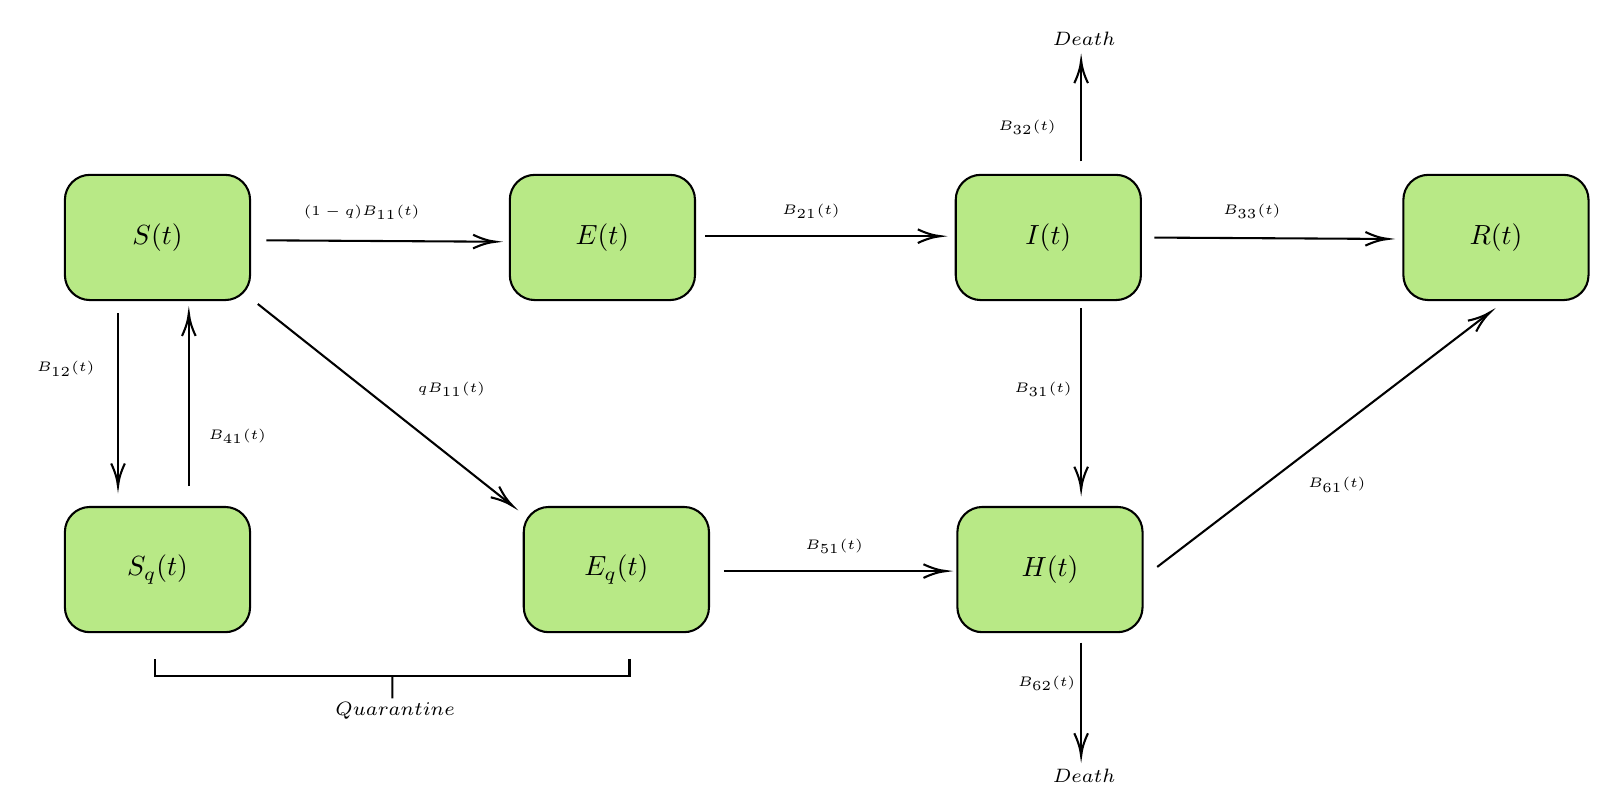
\begin{tikzpicture}[x=0.75pt,y=0.75pt,yscale=-1,xscale=1]
%uncomment if require: \path (0,470); %set diagram left start at 0, and has height of 470

%Rounded Rect [id:dp7623246854359582] 
\draw  [fill={rgb, 255:red, 184; green, 233; blue, 134 }  ,fill opacity=1 ] (85.13,139.47) .. controls (85.13,132.8) and (90.53,127.4) .. (97.19,127.4) -- (162.28,127.4) .. controls (168.95,127.4) and (174.35,132.8) .. (174.35,139.47) -- (174.35,175.67) .. controls (174.35,182.34) and (168.95,187.74) .. (162.28,187.74) -- (97.19,187.74) .. controls (90.53,187.74) and (85.13,182.34) .. (85.13,175.67) -- cycle ;
%Rounded Rect [id:dp4768493132481155] 
\draw  [fill={rgb, 255:red, 184; green, 233; blue, 134 }  ,fill opacity=1 ] (85.13,299.49) .. controls (85.13,292.82) and (90.53,287.42) .. (97.19,287.42) -- (162.28,287.42) .. controls (168.95,287.42) and (174.35,292.82) .. (174.35,299.49) -- (174.35,335.69) .. controls (174.35,342.36) and (168.95,347.76) .. (162.28,347.76) -- (97.19,347.76) .. controls (90.53,347.76) and (85.13,342.36) .. (85.13,335.69) -- cycle ;

%Rounded Rect [id:dp3654569066911406] 
\draw  [fill={rgb, 255:red, 184; green, 233; blue, 134 }  ,fill opacity=1 ] (299.49,139.47) .. controls (299.49,132.8) and (304.89,127.4) .. (311.55,127.4) -- (376.64,127.4) .. controls (383.31,127.4) and (388.71,132.8) .. (388.71,139.47) -- (388.71,175.67) .. controls (388.71,182.34) and (383.31,187.74) .. (376.64,187.74) -- (311.55,187.74) .. controls (304.89,187.74) and (299.49,182.34) .. (299.49,175.67) -- cycle ;

%Rounded Rect [id:dp5762944212255994] 
\draw  [fill={rgb, 255:red, 184; green, 233; blue, 134 }  ,fill opacity=1 ] (306.22,299.49) .. controls (306.22,292.82) and (311.63,287.42) .. (318.29,287.42) -- (383.38,287.42) .. controls (390.05,287.42) and (395.45,292.82) .. (395.45,299.49) -- (395.45,335.69) .. controls (395.45,342.36) and (390.05,347.76) .. (383.38,347.76) -- (318.29,347.76) .. controls (311.63,347.76) and (306.22,342.36) .. (306.22,335.69) -- cycle ;

%Rounded Rect [id:dp021595159630125815] 
\draw  [fill={rgb, 255:red, 184; green, 233; blue, 134 }  ,fill opacity=1 ] (514.33,139.47) .. controls (514.33,132.8) and (519.74,127.4) .. (526.4,127.4) -- (591.49,127.4) .. controls (598.16,127.4) and (603.56,132.8) .. (603.56,139.47) -- (603.56,175.67) .. controls (603.56,182.34) and (598.16,187.74) .. (591.49,187.74) -- (526.4,187.74) .. controls (519.74,187.74) and (514.33,182.34) .. (514.33,175.67) -- cycle ;

%Rounded Rect [id:dp8968884149325778] 
\draw  [fill={rgb, 255:red, 184; green, 233; blue, 134 }  ,fill opacity=1 ] (515.13,299.49) .. controls (515.13,292.82) and (520.53,287.42) .. (527.19,287.42) -- (592.28,287.42) .. controls (598.95,287.42) and (604.35,292.82) .. (604.35,299.49) -- (604.35,335.69) .. controls (604.35,342.36) and (598.95,347.76) .. (592.28,347.76) -- (527.19,347.76) .. controls (520.53,347.76) and (515.13,342.36) .. (515.13,335.69) -- cycle ;

%Rounded Rect [id:dp4560508594384034] 
\draw  [fill={rgb, 255:red, 184; green, 233; blue, 134 }  ,fill opacity=1 ] (730,139.47) .. controls (730,132.8) and (735.4,127.4) .. (742.07,127.4) -- (807.15,127.4) .. controls (813.82,127.4) and (819.22,132.8) .. (819.22,139.47) -- (819.22,175.67) .. controls (819.22,182.34) and (813.82,187.74) .. (807.15,187.74) -- (742.07,187.74) .. controls (735.4,187.74) and (730,182.34) .. (730,175.67) -- cycle ;
%Straight Lines [id:da9482455901186368] 
\draw    (110.72,194.08) -- (110.72,275.42) ;
\draw [shift={(110.72,277.42)}, rotate = 270] [color={rgb, 255:red, 0; green, 0; blue, 0 }  ][line width=0.75]    (10.93,-3.29) .. controls (6.95,-1.4) and (3.31,-0.3) .. (0,0) .. controls (3.31,0.3) and (6.95,1.4) .. (10.93,3.29)   ;
%Straight Lines [id:da05728303880138008] 
\draw    (144.84,277.42) -- (144.84,196.08) ;
\draw [shift={(144.84,194.08)}, rotate = 450] [color={rgb, 255:red, 0; green, 0; blue, 0 }  ][line width=0.75]    (10.93,-3.29) .. controls (6.95,-1.4) and (3.31,-0.3) .. (0,0) .. controls (3.31,0.3) and (6.95,1.4) .. (10.93,3.29)   ;
%Straight Lines [id:da4884708529781723] 
\draw    (357.14,360.65) -- (357.14,368.99) -- (128.72,368.99) -- (128.72,360.6) ;
%Straight Lines [id:da10074852907910814] 
\draw    (242.91,379.65) -- (242.93,368.99) ;
%Straight Lines [id:da11296625559642659] 
\draw    (182.18,158.96) -- (290.73,159.61) ;
\draw [shift={(292.73,159.63)}, rotate = 180.35] [color={rgb, 255:red, 0; green, 0; blue, 0 }  ][line width=0.75]    (10.93,-3.29) .. controls (6.95,-1.4) and (3.31,-0.3) .. (0,0) .. controls (3.31,0.3) and (6.95,1.4) .. (10.93,3.29)   ;
%Straight Lines [id:da37586070655180936] 
\draw    (178.08,189.63) -- (299.35,285.73) ;
\draw [shift={(300.92,286.98)}, rotate = 218.4] [color={rgb, 255:red, 0; green, 0; blue, 0 }  ][line width=0.75]    (10.93,-3.29) .. controls (6.95,-1.4) and (3.31,-0.3) .. (0,0) .. controls (3.31,0.3) and (6.95,1.4) .. (10.93,3.29)   ;
%Straight Lines [id:da7761382576789853] 
\draw    (402.6,318.31) -- (507.73,318.31) ;
\draw [shift={(509.73,318.31)}, rotate = 180] [color={rgb, 255:red, 0; green, 0; blue, 0 }  ][line width=0.75]    (10.93,-3.29) .. controls (6.95,-1.4) and (3.31,-0.3) .. (0,0) .. controls (3.31,0.3) and (6.95,1.4) .. (10.93,3.29)   ;
%Straight Lines [id:da9729894086577398] 
\draw    (393.72,156.96) -- (505,156.96) ;
\draw [shift={(507,156.96)}, rotate = 180] [color={rgb, 255:red, 0; green, 0; blue, 0 }  ][line width=0.75]    (10.93,-3.29) .. controls (6.95,-1.4) and (3.31,-0.3) .. (0,0) .. controls (3.31,0.3) and (6.95,1.4) .. (10.93,3.29)   ;
%Straight Lines [id:da45085066783261496] 
\draw    (574.75,191.63) -- (574.75,276.97) ;
\draw [shift={(574.75,278.97)}, rotate = 270] [color={rgb, 255:red, 0; green, 0; blue, 0 }  ][line width=0.75]    (10.93,-3.29) .. controls (6.95,-1.4) and (3.31,-0.3) .. (0,0) .. controls (3.31,0.3) and (6.95,1.4) .. (10.93,3.29)   ;
%Straight Lines [id:da5455110861418122] 
\draw    (574.75,120.95) -- (574.75,74.28) ;
\draw [shift={(574.75,72.28)}, rotate = 450] [color={rgb, 255:red, 0; green, 0; blue, 0 }  ][line width=0.75]    (10.93,-3.29) .. controls (6.95,-1.4) and (3.31,-0.3) .. (0,0) .. controls (3.31,0.3) and (6.95,1.4) .. (10.93,3.29)   ;
%Straight Lines [id:da20700401454618644] 
\draw    (574.75,352.73) -- (574.75,405.41) ;
\draw [shift={(574.75,407.41)}, rotate = 270] [color={rgb, 255:red, 0; green, 0; blue, 0 }  ][line width=0.75]    (10.93,-3.29) .. controls (6.95,-1.4) and (3.31,-0.3) .. (0,0) .. controls (3.31,0.3) and (6.95,1.4) .. (10.93,3.29)   ;
%Straight Lines [id:da049411173786683804] 
\draw    (611.41,316.31) -- (770.19,194.85) ;
\draw [shift={(771.78,193.63)}, rotate = 502.58] [color={rgb, 255:red, 0; green, 0; blue, 0 }  ][line width=0.75]    (10.93,-3.29) .. controls (6.95,-1.4) and (3.31,-0.3) .. (0,0) .. controls (3.31,0.3) and (6.95,1.4) .. (10.93,3.29)   ;
%Straight Lines [id:da5803439064982177] 
\draw    (610.05,157.63) -- (720.64,158.28) ;
\draw [shift={(722.64,158.29)}, rotate = 180.34] [color={rgb, 255:red, 0; green, 0; blue, 0 }  ][line width=0.75]    (10.93,-3.29) .. controls (6.95,-1.4) and (3.31,-0.3) .. (0,0) .. controls (3.31,0.3) and (6.95,1.4) .. (10.93,3.29)   ;

% Text Node
\draw (129.74,157.57) node   [align=left] {$\displaystyle S( t)$};
% Text Node
\draw (774.61,157.57) node   [align=left] {$\displaystyle R( t)$};
% Text Node
\draw (129.74,317.59) node   [align=left] {$\displaystyle S_{q}( t)$};
% Text Node
\draw (344.1,157.57) node   [align=left] {$\displaystyle E( t)$};
% Text Node
\draw (350.84,317.59) node   [align=left] {$\displaystyle E_{q}( t)$};
% Text Node
\draw (559.74,317.59) node   [align=left] {$\displaystyle H( t)$};
% Text Node
\draw (558.95,157.57) node   [align=left] {$\displaystyle I( t)$};
% Text Node
\draw (228.13,145.62) node  [font=\tiny] [align=left] {$\displaystyle ( 1-q) B_{11}( t)$};
% Text Node
\draw (271.34,230.89) node  [font=\tiny] [align=left] {$\displaystyle qB_{11}( t)$};
% Text Node
\draw (85.46,220.88) node  [font=\tiny] [align=left] {$\displaystyle B_{12}( t)$};
% Text Node
\draw (168.2,253.39) node  [font=\tiny] [align=left] {$\displaystyle B_{41}( t)$};
% Text Node
\draw (213.93,380) node [anchor=north west][inner sep=0.75pt]  [font=\scriptsize] [align=left] {$\displaystyle Quarantine$};
% Text Node
\draw (440.42,301.42) node [anchor=north west][inner sep=0.75pt]  [font=\tiny] [align=left] {$\displaystyle B_{51}( t)$};
% Text Node
\draw (542.78,367.26) node [anchor=north west][inner sep=0.75pt]  [font=\tiny] [align=left] {$\displaystyle B_{62}( t)$};
% Text Node
\draw (548.64,104.62) node  [font=\tiny] [align=left] {$\displaystyle B_{32}( t)$};
% Text Node
\draw (444.57,145.04) node  [font=\tiny] [align=left] {$\displaystyle B_{21}( t)$};
% Text Node
\draw (541.07,225.58) node [anchor=north west][inner sep=0.75pt]  [font=\tiny] [align=left] {$\displaystyle B_{31}( t)$};
% Text Node
\draw (656.97,145.04) node  [font=\tiny] [align=left] {$\displaystyle B_{33}( t)$};
% Text Node
\draw (697.92,276.72) node  [font=\tiny] [align=left] {$\displaystyle B_{61}( t)$};
% Text Node
\draw (559.6,57) node [anchor=north west][inner sep=0.75pt]  [font=\scriptsize] [align=left] {$\displaystyle Death$};
% Text Node
\draw (559.6,412) node [anchor=north west][inner sep=0.75pt]  [font=\scriptsize] [align=left] {$\displaystyle Death$};


\end{tikzpicture}
